\documentclass[USenglish]{article}

\usepackage[utf8]{inputenc}
\usepackage[small]{dgruyter}
\usepackage{microtype}
\usepackage{graphicx}
\usepackage{subcaption}
\usepackage{natbib}
%\graphicspath{ {./images/} }

\begin{document}

  \articletype{...}

  \author*[1]{Lars Pedersen}
  \author[2]{Junni L. Zhang}
  \author[3]{John Bryant} 
  \runningauthor{Lars Pedersen}
  \affil[1]{Statistics Greenland}
  \affil[2]{Peking University}
  \affil[3]{Bayesian Demography Limited}
  \title{Using demographic accounts to enhance official population statistics}
  \runningtitle{ Demographic accounts for Greenland }
  \subtitle{Demographic accounts for Greenland}
  \abstract{...}
  \keywords{...}
  \startpage{1}
  \aop

\maketitle



\section{Introduction} 

A demographic account is the demographic equivalent of a national account. It is a comprehensive description of stocks and flows, linked together by accounting identities, and standardised across countries and datasets. Whereas a national account deals with economic variables such as consumption, savings, and investment, a demographic account deals with demographic variables such as births, deaths, migration, and population. Demographic accounts and national accounts in fact share common intellectual origins. William Petty's political arithmetic, for instance, combined estimates of income and expenditure for 17th century England with estimates of population size. Richard Stone, one of the central figures in the development of modern national accounts wrote extensively on social and demographic accounting, and devoted the final part of his Nobel Prize acceptance speech to subject of demographic accounts. REFERENCES.

National accounts and demographic accounts have, however, followed very different institutional trajectories. National accounts are the centerpiece of official economic statistics. National accounting terms such as ``Gross Domestic Product'' or ``trade surplus'' are used routinely, not just by economists and statisticians, but by newspapers, politicians, and the general public. Detailed guidelines on the compilation of national accounts have been prepared by bodies such as the United Nations and the European Union. REFERENCES. Although some standardised demographic tabulations such as the United Nations \emph{World Population Prospects}, or population estimates and projections produced by national statistical agencies, are widely used and discussed, they do provide enough detail to permit detailed accounting. Scholars from a variety of disciplines have developed conceptual frameworks and estimation methods for demographic accounts \citep{rees1977spatial,rees1986data, rees1979regional,rees1985choices,rees2012ethnic,bryant2013bayesian, wheldon2013reconstructing,willekens2011population} OTHER. However, no set of guidelines have achieved the same prominence or adherence as the official guidelines for national accounts.  Moreover, the terminology and techniques of demographic accounting are not well known, even among statisticians and demographers.

In this paper we argue that the adoption of formal demographic accounting could help improve the clarity, consistency, and ease of use of official population statistics. We illustrate using the case of Greenland, which already publishes official demographic accounts. ROAD MAP FOR PAPER.

[Need that Stone's original social and demographic accounts had more than just basic demography]


\section{What is a demographic account?}

\begin{quote}
Demographic accounts, like any other type of account, are based on the equality of inflows and outflows over a period of time. In the demographic case, the inflows and outflows are composed of human beings \citep[][p. 26]{stone1984accounts}.
\end{quote}

A demographic account is a set of linked tabulations of demographic stocks and flows. The stocks and flows that are included in the account, and the ways that the stocks and flows are classified, vary from application to application. In all cases, however, the stocks and flows are linked via the accounting identity
\begin{equation*}
    \text{change in stock} = \text{inflows} - \text{outflows}.
\end{equation*}
We illustrate the underlying principles using some stylised examples, before presenting an extract from a full scale official account for Greenland.

An example of a minimal demographic account is
\begin{center}
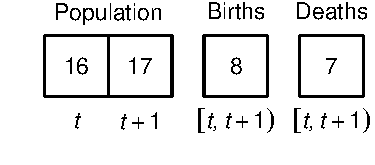
\includegraphics[width=0.3\textwidth]{figures_accounts/fig_account_noage.pdf}
\end{center}
The population contains 16 people at time $t$ and 17 people at time $t+1$; during the interval between $t$ and $t+1$, 8 people are born and 7 die. The change in stock,
\begin{equation*}
  17 - 16 = 1,
\end{equation*}
equals inflows minus outflows,
\begin{equation*}
   8 - 7 = 1,
\end{equation*}
as required. There is only one accounting equation, since the account treats the population as completely homogenous, with everyone belonging to a single group.

Most demographic accounts divide the population into multiple groups. The following account recognizes two groups, labelled ``A'' and ``B''. 
\begin{center}
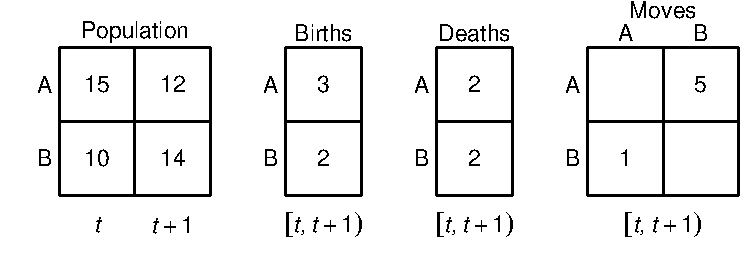
\includegraphics[width=0.55\textwidth]{figures_accounts/fig_account_region.pdf}
\end{center}
A and B could, for instance, denote geographical region, health status, or labour force status. In this example, we assume that people can change their status from A to B and vice versa.

Demographic accounting can be done for the population as a whole,
\begin{equation*}
    17 - 16 = 8 - 7,
\end{equation*}
in which case movements between A and B do not appear, since they do count as inflows to or outflows from the population as a whole. Demographic accounting can also be done for each group,
\begin{align*}
    8 - 10 & = 3 - 4 - 7 + 6 \quad \text{(A)}\\
    14 - 10 & = 5 - 3 - 6 + 7 \quad \text{(B)},
\end{align*}
in which case movements between A and B do appear. The 7 movements from A to B show up twice in the account, once as a decrement from group A, and once as an increment to group B. Similarly, the 6 movements from B to A show up as a decrement from B and as an increment to A.

One particular type of disaggregation has a special status within demography: disaggregation by age group. Age is special because it is such a strong predictor of demographic behavior. The mortality and migration rates of 20-24 year olds and 90-94 year olds, for instance, differ by several orders of magnitude. Age is also special because movement between age groups is deterministic. Everyone is born into the lowest age group and then moves upwards at the rate of one age group per period.

Producers of age-structured demographic data typically present some variant on the format
\begin{center}
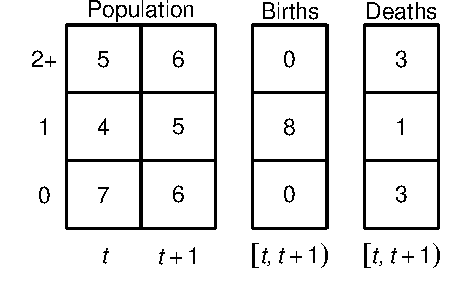
\includegraphics[width=0.45\textwidth]{figures_accounts/fig_account_withage_nolex}
\end{center}
For simplicity, the diagram here only shows three age groups, labelled ``0'', ``1'', and ``2+''. Actual tabulations typically include more age groups and time periods, and disaggregate by additional dimensions such as sex or gender.

The standard format for age-structured demographic data does not include enough information to permit detailed demographic accounting. The format does allow accounting for the population as a whole. We are able to calculate changes in stocks
\begin{equation*}
    (6+9+8)-(5+4+7) = 23 - 16 = 7,
\end{equation*}
and inflows minus outflows, 
\begin{equation*}
    (0+7+0)-(7+1+3)+(5+7+7)-(3+5+1) = 7 - 10 + 19 - 9 = 7,
\end{equation*}
and check that they are the same. The format does not, however, allow us to do demographic accounting within age groups. 

Consider what happens, for instance, when we try to apply demographic accounting to individuals who were aged 0 at time $t$. Calculating the change in stock for these individuals is easy. Individuals who were aged 0 at time $t$ are aged 1 at time $t+1$. The change in stock is therefore 9 - 7 = 2. Calculating inflows and outflows, however, is more difficult. Individuals who were aged 0 at time $t$ are presumably responsible for some of the 3 deaths, 7 immigrations, and 1 emigration that occur to 0 year olds during the period $[t,t+1)$. However, it is impossible to tell exactly how many, since since some of the events could also have occurred to individuals who were born during the period. Similarly, individuals who were aged 0 at time $t$ are presumably responsible for some of the 7 births, 1 death, 7 immigrations, and 5 emigrations that occur to 1 year olds during the period. But once again it is not possible to tell exactly how many, in this case because some of the events may have occurred to individuals who were already aged 1 at time $t$.
Without the ability to calculate inflows and outflows for individuals aged 0 at time $t$, we cannot do demographic accounting for this group.

Groups such as ``individuals aged 0 at time $t$'', ``individuals born during period $[t, t+1)$'', and ``individuals aged 1 at time $t$'' are examples of birth cohorts, that is, collections of individuals all born during the same period. Cohorts always appear in some form in demographic accounting involving age, since, to relate stocks at one period to stocks at another period, we need to follow cohorts. The fundamental obstacle to doing demographic accounting with standard formats like the one above is that the formats do not contain enough information to unambiguously assign events to cohorts.

To remove the ambiguity, each combination of age and period needs to be split into two. We need to be able to distinguish between
\begin{enumerate}
    \item events experienced by the cohort that belongs to age group $a$ at the start of the period, and
    item events experience by the cohort that enters age group $a$ during the period.
\end{enumerate}
Demographers refer to the first set of events as belonging to `upper Lexis triangles' and refer to the second set of events as belonging to `lower Lexis triangles'.

The diagram below expands on the previous one by adding a distinction between Lexis triangles.
\begin{center}
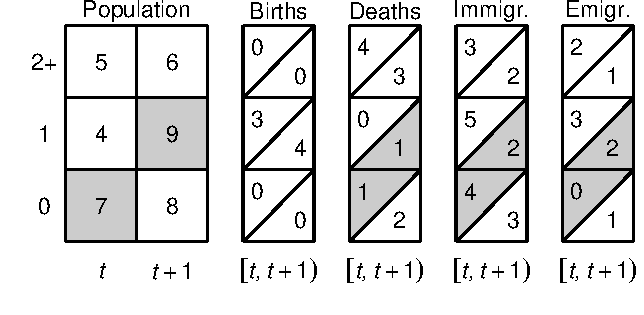
\includegraphics[width=0.5\textwidth]{figures_accounts/fig_account_withage_lex.pdf}
\end{center}
Consider again the cohort aged 0 at time $t$. With Lexis triangles now shown, we can see that the cohort aged 0 at time $t$ experienced 1+1 deaths, 4+2 immigrations, and 0+2 emigrations, for a total inflow of 6 and outflow of 4, which is consistent with a change in stock of 2.

Births have a special status within a demographic account that includes age. Births involve two people: the person having the birth, and the person being born. In a demographic account that includes age, births are typically tabulated by the age of the person having the birth, not the age of the person being born, which is always zero. Births appear in demographic accounting as a type of starting population, for the cohort being born. 

For the cohort that is born during the period $[t,t+1)$ in our diagram, the starting population is obtained by adding up over the age and cohort of the parent:
\begin{equation*}
    0 + 0 + 3 + 4 + 0 + 0 = 7.
\end{equation*}
The change in stock is
\begin{equation*}
    8 - 7 = 1.
\end{equation*}
The 
Analogous calculations can be carried out for other cohorts:,
\begin{align}
    8 - (3 + 4) & = -2 + 3 - 1 & \text{(Born during $[t,t+1)$)} \\   
    9 - 7 & = -(1 + 1) + (4 + 2) - (0 + 2) & \text{(Age 0 at $t$)} \\
    6 - (5 + 4) & = -(0 + 3 + 4) + (5 + 2 + 3) - (3 + 1 + 2)  & \text{(Age 1+ at $t$)}
\end{align}
(Following standard demographic practice, we combine the two oldest cohorts to obtain values for the open-ended age group.)

PRESENT GREENLAND EXAMPLE.


\section{Greenland demographic data}

\subsection{Population Register from 1973} 

(Statistics Denmark published detailed Population Accounts with [Lexis-triangles]("Befolkningens Bevægelser") on paper from 1964-2004)

Statistics on the Greenlandic population are all based on information in administrative registers with 100 pct national coverage. The base register (CPR) was introduced to Greenland in 1972 and in effect for statistical purposes from 1977. All daily changes to the population’s addresses are recorded, by law, no later than 5 weekdays after occurrence and correctly. This would be a perfect data dream, which in real life, never happens. Even in a ultra small society as the Greenlandic, many hundred persons add changes to the central register annually, so of cause errors are reported, as also events are reported with some delay.

Some events, especially on external migrations are reported more than a year after actual occurrence. Some very few death are also reported very late. According to law, a court can issue a death certificate declaring ‘presumption of death’ of a missing person, no earlier than 10 years after the person disappeared.



\section{Greenland demographic account}

The Population Account for Greenland offers a set of coherent tables that allows calculations of all demographic measures at aggregated level.

A core table holds totals of demographic events that  explains annual change in the population size. The sum of birth surplus and net migration makes up the difference in annual population estimates, but will only be accurate in a world with perfect data. In all practical situations there need to be a hopefully small correction figure added, to make the account coherent. At the same time, analysis of corrections offers valuable information on possible data problems, Statistics Greenland should aim to improve.

The account can be broken down in categories like ‘place of birth’, sex and region and also from three variables ‘year of birth’, time and lexis-triangle, age can be calculated. 

This is a sufficiently detailed table to serve as a model of the Greenlandic population ready to be consumed for descriptive purposes or as baseline in projections.

At national level totals of net internal migration is per definition equal zero, but in regional forecasts movings between regions are essential in order to predict the size, sex and age distribution in the regions. Instead of adding dimensions on origin and destination to the core account, a satellite table focus on internal migrations.

The same goes for number of live born. They too are accessible in a satellite table with dimensions ‘sex of child’ and on mother: ‘place of birth’, ‘year of birth’, age, region and time.



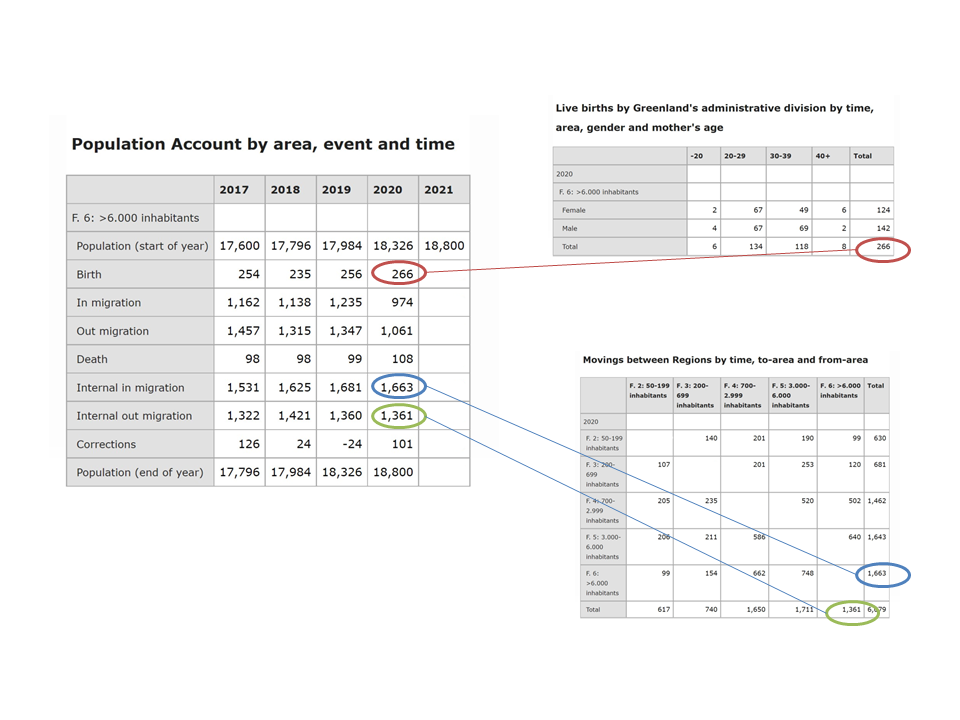
\includegraphics[scale=0.4]{images/PopulationAccountCoreSatellite}

category dimensions (sex, place of birth) can be filtered some with alternate classifications

other fixed category dimensions could be relevant: 

categories changing over time:
citizenship, education, income, marital status


\subsection{Dimensions in core table} 
The central dimension in the core table is called ‘event’ eventhough it also holds population estimate at start and end of year. Population at start of year plus the sum of net-events equals population at end of year/start of the following year.

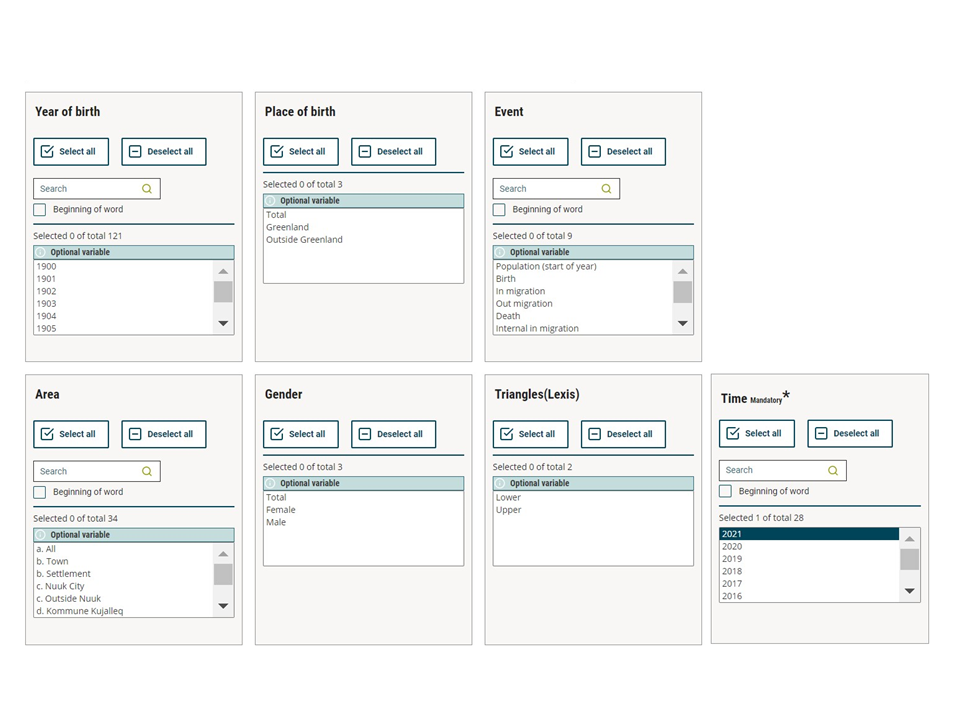
\includegraphics[scale=0.4]{images/PopulationAccountCore}
Filter dimensions are: area, ‘Place of Birth’ and gender, but the Greenlandic statistical system could provide altenate dimensions like ancestry, education, marital status, income


\subsection{Age at event} 

The Statbank Greenland, core table does not have an age dimension, instead age-at-event has to be calculated from ‘year of birth’ (cohort) and time (period) as time dimensions.

To allow calculation at time of event a ‘triangles(lexis)’-dimension is provided. This enables calculation of age, at time of event. The vertical parallelogram counts events that are defined by calendar year and year of birth (cohort) - accross 2 agespans. Knowing that events occured before or after a persons birthday in a calendar year, is needed to calculate persons age at event, but then is easily calculated:

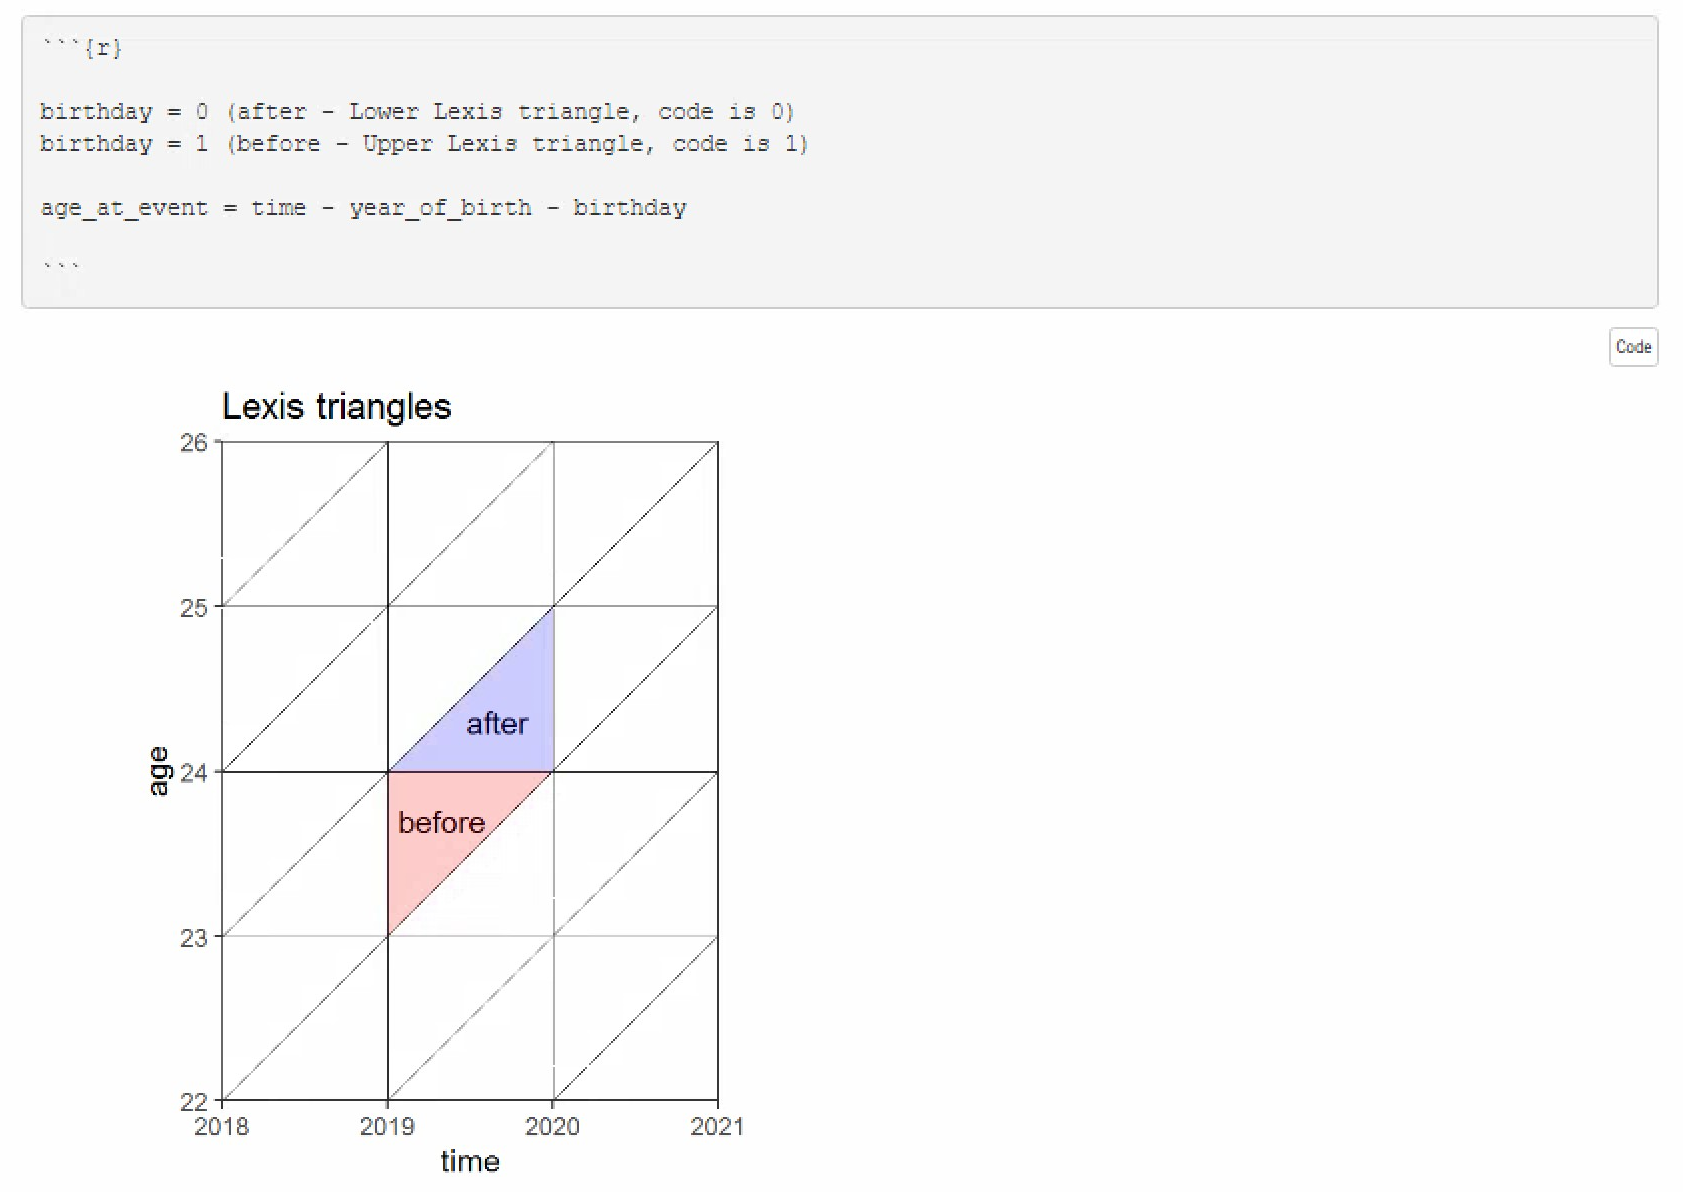
\includegraphics[scale=0.25]{images/PopulationAccountLexis}


(Lars: columns are not in right sort-order!)

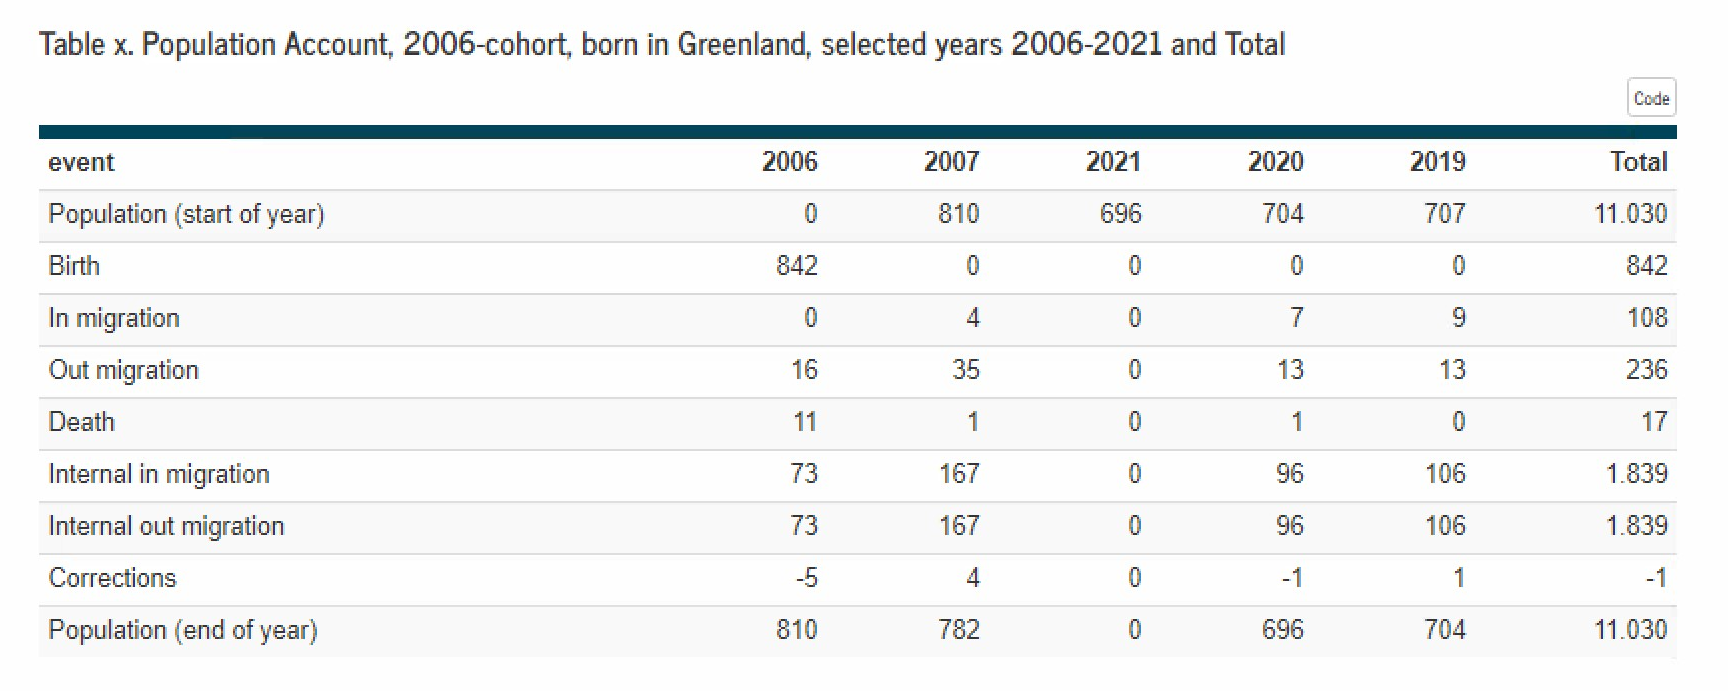
\includegraphics[scale=0.22]{images/PopulationAccountTabX}


To be up to date (timely?) and of use to society statistics can not wait being 100 pct accurate. Instead we settle when the statistics are true and fair. From experience it has been chosen to wait 1 calendar month, to allow the register to be updated with delayed reports. Then the population estimate is adjusted to include events taken place before the report date, January 1st. (or other dates chosen). As long as the number of delayed reported events are approximately the same from one period to the next, the number of events will be approximately equivalent.

But on detailed level (one-year age groups, gender, locality) this will not be true.

Changes in P(opulation) size are described by the vital statistics: B(irths), D(eaths), I(mmigrations) and E(migrations). But because of the delayed reports, a residual calculated c(orrection) post is added to ensure


P(t+1) = P(t) + B(t) - D(t) + I(t) - E(t) + c(t)


For subnational population calculations internal migration is simply added to this equation.

The correcton post offers important quality information on how well the vital statistics explains changes in population size over time.

As the content is not 100 pct accurate, but true and fair, this serves as a model of the Greenlandic population


\subsection{Statbank Greenland} 
Statistics Greenland has been disseminating statistical tables with Pxweb as multilingual internet based service since 2001. The technical core is \footnote[the Pxweb-family]{https://www.scb.se/px-web}, primarily developed by Statistics Sweden in cooperation with approximately 40 national statistical offices over a span of 5 decades. 

In 2013 the system opened for api access. As proof of concept www.stat2go.com gives access to a number of national pxweb-based statbanks, where the api allows developers to reuse and include statistical information in solutions, whether they have commercial ambitions (like knoema.com, statista.com) , supports fact-based documents for knowledge and/or research .

For the R-community CRAN-published packages bridge tables from national statistical institutes directly to statistical analysis. As example Population Accounts from both Greenland and the Faroe Islands can be obtained with some few lines of code, ready for analysis.

The pxweb package includes functionality to generate needed r-code from many datasources. The function call is pxweb\_interactive.


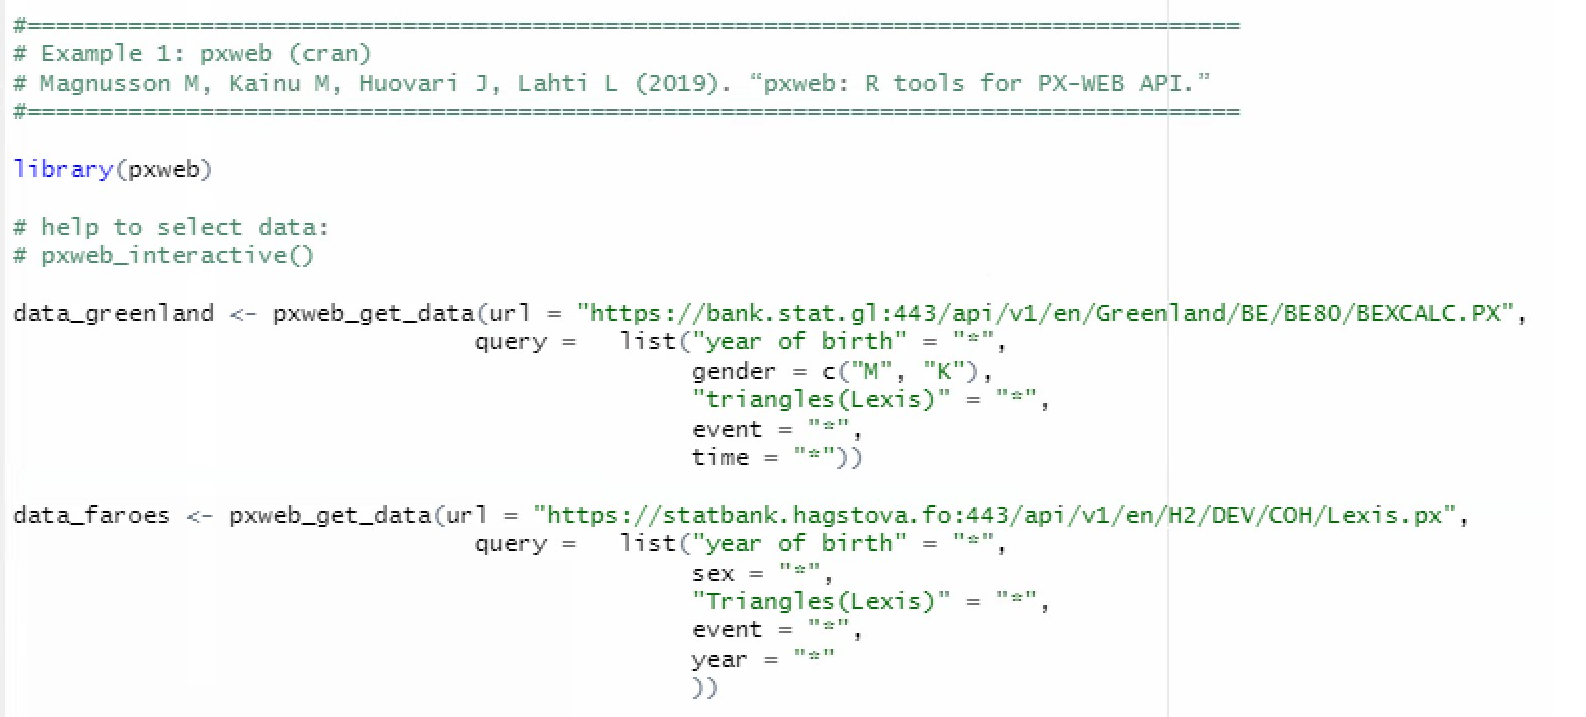
\includegraphics[scale=0.22]{images/pxwebR_GF.png}


Reference: Magnusson M, Kainu M, Huovari J, Lahti L (2019). “pxweb: R tools for PX-WEB API.”


\section{Discrepancies}

\subsection{What are discrepancies}



\subsection{How inconsistencies occur}

Corrections are residuals, calculated to balance the sum of events in any period to explain change in the periodic population estimate.

No statistical office can produce a 100 percent correct population account, without any adjustment. Statistics Greenland has chosen, not to adjust, not to hide data discrepancies. Instead corrections are treated as vital quality information on the collection/production system.

Errors and data discrepancies are as natural as birth and death, and analysis of the discrepancies can help in search for possible improvements.

First of all discrepancies can be caused by for instance: a) Some registrations in the population register are not considered. The register holds information on persons gone missing, and being refound b) The administrative register is updated by humans, not always knowing the full truth. Typos, errors and better information can lead to multiple updates to the same event. To lower complications when calculation, not all corrections are used c) Statistics Greenland only take into account, events that have been reported no later than one calendar month after the period ends.

a and b could be improved, but a short cost/benefit has given this extremely low priority. c is no problem at aggregate level, if reports of future events not known at the time of production are more or less equal to the latecomming reports from previous years. Compared with results of longetutional analysis there will be small discrepancies. But that is the name of the game.

When corrections are summarized over time they diminish. In table x the corrections for the 2006-cohort is down to -1 over a 15 year period. 

\subsection{Methods to eliminate discrepancies}

\subsubsection{Pure expert judgement}

\citep{lomax2013subnational}


\subsubsection{Quality-based weights}




\subsubsection{System models and data models}

\citep{bryant2013bayesian} \citep{wheldon2013reconstructing}\citep{wheldon2015bayesian}

\begin{figure}
    \centering
    \begin{subfigure}{\textwidth}
    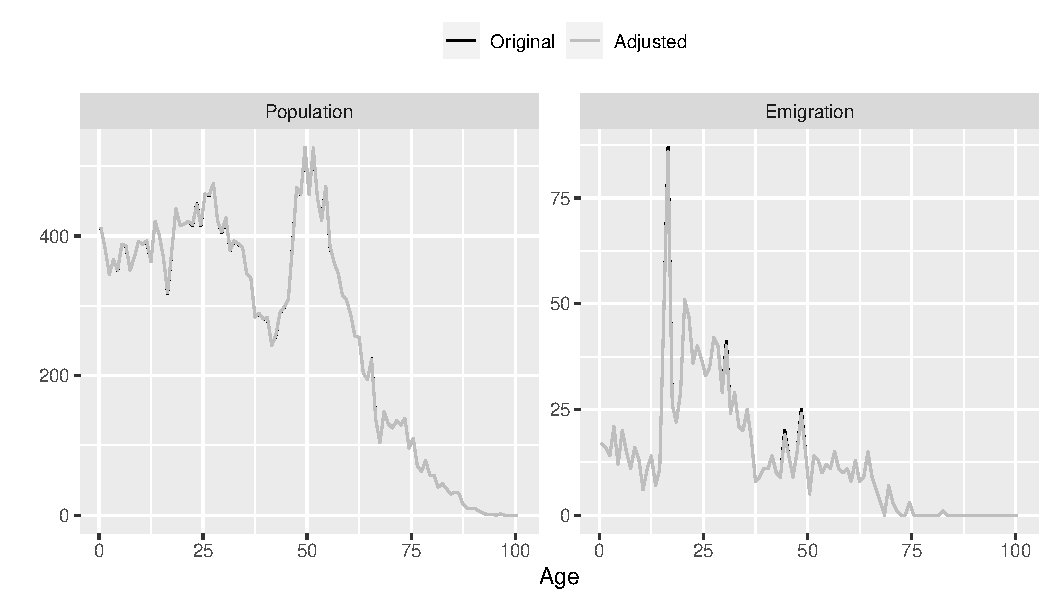
\includegraphics[width=\textwidth]{estimate_account/out/fig_values}
    \caption{Original and adjusted values}
    \end{subfigure}
    \begin{subfigure}{\textwidth}
    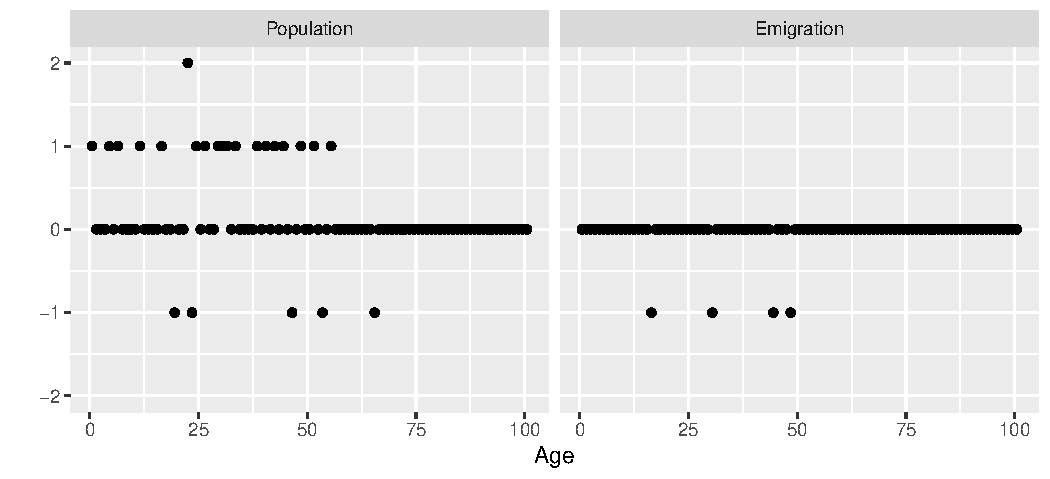
\includegraphics[width=\textwidth]{estimate_account/out/fig_diff}
    \caption{Differences between original and adjusted values}
    \end{subfigure} 
    \caption{Adjustment of Greenland account, using Bayesian demographic accounts. The upper panels show illustrative results for females, for two components of the account, in 2015. The lower panels show the size of the differences between original and adjusted values. See the text for a description of the model.   }
    \label{fig:my_label}
\end{figure}


\clearpage


\section{Benefits of a demographic account}

\begin{itemize}
    \item data corrections (note - will discuss further below)
    \item understanding Greenland demographic system (eg movements to/from Denmark)
    \item transparency eg in forecasting
    \item make it easy for people to get data on demographic change, all in one place - and understand
    \item better scenario analysis
\end{itemize}



\section{Dissemination}

\begin{itemize}
    \item stat bank system
    \item ease of getting data
    \item common conventions on what the data should look like (to go with common software)
    \item how to disseminate uncertainty?
\end{itemize}

\section{Discussion (implications for other countries)}

\begin{itemize}
    \item can other countries emulate Greenland?: countries with good data vs countries with bad data
    \item why is it also useful in other countries
    \item can countries without population registers emulate greenland
    \item many agencies do accounting implicitly, adhoc
    denmark published on paper from 1964-2004, then stopped ) :
    \item accounts for holland, faroe islands
    
\end{itemize}

What about countries without population registers?
\begin{itemize}
    \item a population count is a *model* of the population
    \item if a country does not have a population register but can estimate it, then they can still do an account; and reconcile via stat method
    \item need to be transparent but it best that can be produced
    \item we use National Accounts - even though they are badly imperfect
    \item in Copenhagen, demographic accounts where part of the demography mainstream
\end{itemize}


\begin{acknowledgement}
  ...
\end{acknowledgement}

\bibliographystyle{apalike}
\bibliography{references}{}

\end{document}



******************** NOTES *************************************


- we are assuming good-quality (even if not perfect) input data
- including full details of age and cohorts
- we will focus on countries with good quality data (though we believe that demographic accounts also useful for countries with poor data)


target audience: official statistics agencies in countries with good data

outline of paper
- introduction
  - demographic accounts have same origin as national accounts
  - have same advantages - eg common format, framework, accounting identities to infer missing quantities
  - but demography has better data!
    - motivating example: greenland 
    - why greenland?
        - because has published account - automated, API
        - much more detailed and integrated than most (because has Lexis triangles)
     - main advantage: standard format that can be used for many purposes, same format for forecasts, modelling, all different series, cross-country comparison, non-demographic variables [sex, region, place of birth categories  - but also income, education, occupation] - cite Richard Stone
    - although we consider more widely
- greenland data (or countries with population registers??)
  - raw data
  - processed data
- *published* account for greenland
  - very aggregated
  - national
  - subnational
- why it is useful (for greenland)
    - data corrections (note - will discuss further below)
    - understanding Greenland demographic system (eg movements to/from Denmark)
    - transparency eg in forecasting
    - make it easy for people to get data on demographic change, all in one place - and understand
    - better scenario analysis
 - dealing with inconsistencies
    - including 'corrections' in account (analogous to national account)
    - can use estimation methods to make it consistent
       - maybe give example using 'demest'?? (small example)
  - dissemination
     - stat bank system
     - ease of getting data
     - common conventions on what the data should look like (to go with common software)
     - how to disseminate uncertainty?
  - discussion: implications for other countries
    - can other countries emulate Greenland?
       - countries with good data
       - countries with bad data
    - why is it also useful in other countries
    - can countries without population registers emulate greenland
    - many agencies do accounting implicitly, adhoc
    denmark published from 1975-2004, then stopped ) :
    - accounts for holland, faroe islands
    
    
    - 
- 
- 



FOCUS OF PAPER

opening statement? why this paper?

greenland has registerbased, almost perfect data to model its population and publish detailed data, accessible by api in a popacc.

for countries with less detailed data a popaccount on local level can be estimated using bayes methods demonstrated with project greenlandaccount 

the methods can be compared with the greenlandic data  

no matter how a country's pop is estimated, the popacc can serve as a full repository for all demograhic meassures and forecasts. in most stat offices the info is gathered by many specialized employees, the popacc will bring this knowledge together




- arguments [and good showcases] for demographic accounts

larp: from the popaccount I now extract data that serve as input to mortality.org step 2, generates HMD data tables, step 3 run all code that uses this format. 

- to convince countries we have to show that they can be used

- Nico Kielman: does not need account because he gets the data anyway
- places like HMD very specific in their focus
- HFD is another project
- to do forecasts need more info
- need general way to have population accounts - then others would use them
- lots of interest in local level details
- demographic accounts are likely to be useful for local level


- iceland migration paper
   - Lars reproducing with Greenland data
   - internal migration could be included in account with satellite table
   - could add origin-destination to core regional table
   - fertility could be a satellite table with mother's age
- applications of regional accounts
   - population forecasts
   - regional analyses of mortality
   - 
- lots of interest in local demographic change
    - to understand need to have all components of change
    - need to present data in a form that people can download and look at themselves
    
- Lars wants to do non-black box forecasts for Greenland, including publishing the code on github
- it can be hard for people to get hold of data - hasn't improved since the 1990s

larp: the technical possibilities have exploded. api's in place for 5 years now. cannot remember this argument. 

- pxweb - accessible data - include this as a part of the wider package of a 'demographic account'

infrastructure
- data collection (popn registers in Greenland)
- reconciliation
- public dissemination

Nordic countries - can combine everything via personal ID

What about countries without population registers?
- a population count is a *model* of the population
- if a country does not have a population register but can estimate it, then they can still do an account; and reconcile via stat method
- need to be transparent but it best that can be produced
- we use National Accounts - even though they are badly imperfect
- in Copenhagen, demographic accounts where part of the demography mainstream

the Danish Population account on national level was published from 1975 to 2004 on paper. 

a lot of demographic accounting is implicit

- in nordic countries individual-level data is available - everyone concentrates on that

- don't need individual-level data for accounts

- demographic analyses are tied to aggregate-level analysis
- advantages of aggregate-level analysis
   - does not invade privacy, can be transparent
   - some processes, concepts are intrinsically aggregate - eg demographic

- account has to be designed to be meaningful for the society
- what variables are included etc
- dimensions will vary from place

- Why is Eurostat not interested in demographic accounts?
    - want to gather info at disaggregated level with Lexis triangles
    - Eurostat is doing something (UNIDEMO)
    - 

Why bother with Lexis triangles
- if we have the data, then we can do all theoretical possible ways of calculating life expectancy - more refined indicators
- there are some indicators of interest that are related to cohorts - eg cohort fertility, mortality
- need cohorts/triangles to make translation between period and cohort nicely - if you have the data, then why not use it; if you are modelling, it is best to be explicit
- differences may be small empirically; 
- you should publish both cohort and age views
- publishing both means that it is not a black box
- can't assess internal consistency without looking at cohorts
- cohorts are neglected social unit - we want make it easy to calculate chorts  - it is painful or impossible to calculate (they are not transparent) 
- get most value from data


- Are Lexis triangles too hard
- How old am I?
   - Lexis triangle shows us how to calculate how old we are
   - 




If we have standard format for demographic data, then we can have standard/generic models - just like with demographic accounts

Most countries already have demographic accounts - we want them to make the accounts more standard and detailed - so they are comparable

Greenland is the example
- 


Denmark did demographic accounts with Lexis triangles in 1964 by hand 
- they stopped in 2005, when transferring to the statbank, but never included in statbank
- why did Denmark do demographic accounts? Used in calculation of life expectancy


with big data era, big tables is no big deal - provided that data is standardised

look at the example of HMD - having standardized detailed data for many countries has had huge impact on the study of mortality


- Stone's social and demographic accounts looked at non-demographic variables
- these could be useful for Stats agencies - eg demographic accounts for labour market

- Greenland - linelines. Data automatically internally consistent
- Nordic countries have this amazing data that allows lifelines
- researchers allowed to access, with lots of privacy restriction

- discussion: start with demographic variables, and then move to other social/economic variables
- demographic variables are simpler
- core demographic account is baseline to all projection
   - demographic variables are foundation for other parts
   - have satellite tables
- if a demographic account is available to researchers, they can build their own projections
- they can try lots of different methods and solutions
- can compare and share ideas across countries


why did demographic accounts die out in 1970s 1980s?
- perhaps too difficult to deal with big numbers (with their limited budgets)
- maybe statistical methods not up to the job
- Nordic countries wrote their theory only in Danish etc
- demographic accounting done in stats agencies
    - stats agencies are not good at documenting what they do
    - no accumulation, critical mass 
    - 
- 